% cpedoc.tex V2.0, 13 May 2010

\documentclass[times]{cpeauth}

\usepackage{moreverb}
\usepackage{xspace}

\newif\ifdraft
\drafttrue
\ifdraft
\newcommand{\onote}[1]{ {\textcolor{cyan} { (***Ole: #1) }}}
\newcommand{\terminology}[1]{ {\textcolor{red} {(Terminology used: \textbf{#1}) }}}
\newcommand{\owave}[1]{ {\cyanuwave{#1}}}
\newcommand{\jwave}[1]{ {\reduwave{#1}}}
\newcommand{\alwave}[1]{ {\blueuwave{#1}}}
\newcommand{\jhanote}[1]{ {\textcolor{red} { ***shantenu: #1 }}}
\newcommand{\alnote}[1]{ {\textcolor{green} { ***andreL: #1 }}}
\newcommand{\amnote}[1]{ {\textcolor{blue} { ***andreM: #1 }}}
\newcommand{\smnote}[1]{ {\textcolor{brown} { ***sharath: #1 }}}
\newcommand{\pmnote}[1]{ {\textcolor{blue} { ***Pradeep: #1 }}}
\newcommand{\msnote}[1]{ {\textcolor{cyan} { ***mark: #1 }}}
\newcommand{\note}[1]{ {\textcolor{magenta} { ***Note: #1 }}}
\else
\newcommand{\onote}[1]{}
\newcommand{\terminology}[1]{}
\newcommand{\owave}[1]{#1}
\newcommand{\jwave}[1]{#1}
\newcommand{\alnote}[1]{}
\newcommand{\amnote}[1]{}
\newcommand{\athotanote}[1]{}
\newcommand{\smnote}[1]{}
\newcommand{\pmnote}[1]{}
\newcommand{\jhanote}[1]{}
\newcommand{\msnote}[1]{}
\newcommand{\note}[1]{}
\fi

\usepackage{color}

\usepackage{listings}  
\lstdefinestyle{myListing}{
  frame=single,   
  %float=t,
  language=C,       
  basicstyle=\ttfamily \footnotesize,
  breakautoindent=true,
  breaklines=true
  tabsize=2,
  captionpos=b,  
  aboveskip=0em,
  belowskip=-2em,
  %numbers=left, 
  %numberstyle=\tiny
}      

\lstdefinestyle{myPythonListing}{
  frame=single,   
  %float=t,
  language=Python,       
  basicstyle=\ttfamily \footnotesize,
  breakautoindent=true,
  breaklines=true
  tabsize=2,
  captionpos=b,  
  %numbers=left, 
  %numberstyle=\tiny
}

\newcommand{\cloud}{cloud\xspace}
\newcommand{\clouds}{clouds\xspace}
\newcommand{\pilot}{Pilot\xspace}
\newcommand{\pilots}{Pilots\xspace}
\newcommand{\pilotjob}{Pilot-Job\xspace}
\newcommand{\pilotjobs}{Pilot-Jobs\xspace}
\newcommand{\pilotcompute}{Pilot-Compute\xspace}
\newcommand{\pilotdata}{Pilot-Data\xspace}
\newcommand{\pilotdataservice}{Pilot-Data Service\xspace}
\newcommand{\pilotcomputeservice}{Pilot-Compute Service\xspace}
\newcommand{\computedataservice}{Compute-Data Service\xspace}
\newcommand{\pilotmapreduce}{PilotMapReduce\xspace}
\newcommand{\pd}{PD\xspace}
\newcommand{\pj}{PJ\xspace}
\newcommand{\pjs}{PJs\xspace}
\newcommand{\pds}{Pilot Data Service\xspace}
\newcommand{\computeunit}{Compute-Unit\xspace}
\newcommand{\computeunits}{Compute-Units\xspace}
\newcommand{\dataunit}{Data-Unit\xspace}
\newcommand{\dataunits}{Data-Units\xspace}
\newcommand{\du}{DU\xspace}
\newcommand{\dus}{DUs\xspace}
\newcommand{\cu}{CU\xspace}
\newcommand{\cus}{CUs\xspace}
\newcommand{\su}{SU\xspace}
\newcommand{\sus}{SUs\xspace}
\newcommand{\schedulableunit}{Schedulable Unit\xspace}
\newcommand{\schedulableunits}{Schedulable Units\xspace}
\newcommand{\cc}{c\&c\xspace}
\newcommand{\CC}{C\&C\xspace}

\usepackage[
%dvips,
colorlinks,bookmarksopen,bookmarksnumbered,citecolor=red,urlcolor=red]{hyperref}

\newcommand\BibTeX{{\rmfamily B\kern-.05em \textsc{i\kern-.025em b}\kern-.08em
T\kern-.1667em\lower.7ex\hbox{E}\kern-.125emX}}

\def\volumeyear{2012}

\begin{document}

\runningheads{A. Luckow et al.}{Pilot-Abstractions for MapReduce-based  Cloud Applications}

\title{Pilot-Abstractions for MapReduce-based Cloud Applications}

%on Clouds and Grids}

%Extensible, Scalable, Interoperable 

\author{Andre Luckow, Pradeep Mantha, Melissa Romanus, Shantenu
  Jha\corrauth}

\address{Radical Research Group, Rutgers University}

\corraddr{Journals Production Department, John Wiley \& Sons, Ltd,
The Atrium, Southern Gate, Chichester, West Sussex, PO19~8SQ, UK.}

\begin{abstract}
% The data generated by scientific applications is experiencing an
% exponential growth. Addressing the consequences of this exponential
% growth has spawned the field of BigData. Given that data and compute
% resources cannot always be co-located, an important component of the
% BigData problem is how to utilize the efficient use of distributed
% resources so as to make meaningful sense of all of the data produced.
% In recent work we showed how MapReduce can be used to efficiently
% process distributed data across a distributed set of resources.
% Pilot-MapReduce (PMR) is a flexible, infrastructure-independent
% runtime environment for MapReduce. PMR is based on \pilot-abstractions
% for compute (Pilot-Jobs) and data (Pilot-Data). Pilot-Jobs are used to
% couple the map phase computation to the nearby source data, and
% Pilot-Data is used to move intermediate data using parallel data
% transfers to the reduce computation phase.

  The data generated by scientific applications is experiencing an
  exponential growth. The ability to analyze prodigious volumes of
  data require efficient compute-data co-placement.  Capabilities such
  as runtime environments and methods that support scalable yet
  flexible analytical approaches are required.  This paper proposes
  the use of Pilot-abstractions as one way to achieve such flexible
  usage of clouds.  In particular, we focus on Pilot-Data and the use
  of clouds as one element in a broader and heterogeneous distributed
  cyberinfrastructure.  To that end, we build upon existing
  capabilities of integrating MapReduce with \pilot-abstractions (called
  Pilot-MapReduce (PMR)). PMR is based on \pilot-abstractions for
  compute (Pilot-Jobs) and data (Pilot-Data) and provides a flexible,
  infrastructure-independent runtime environment for MapReduce.
  Pilot-Jobs are used to couple the map phase computation to the
  nearby source data, and Pilot-Data is used to move intermediate data
  using parallel data transfers to the reduce computation phase.  In
  this paper, we discuss the generalization of the pilot-abstraction
  to clouds and investigate the use of PMR on a variety of cloud
  systems, as well as interoperably with other distributed resources.
  We show how Pilot abstractions and PMR enable the efficient
  processing of distributed data on heterogeneous distributed
  infrastructure including different academic and commercial clouds
  (e.g. Amazon EC2, Google Compute Engine and FutureGrid). We
  investigate the effectiveness of PMR based applications on cloud
  infrastructure for different next-generation gene sequencing
  applications.  The flexible runtime provided by the
  Pilot-abstraction, helped establish PMR's effectiveness for
  distributed data scenarios on clusters that are nodes on a
  WAN. Given the different network characteristics within clouds, we
  investigate whether performance determinants for clusters, are valid
  for clouds.  We analyze different resource and MapReduce
  configurations, such as both hierarchical and distributed MapReduce
  using an NGS application.  Our analysis covers multiple scenarios
  exposing the different (typical) trade-offs: e.g., the overhead
  times in spawning virtual machines, different storage types,
  geographic distribution, and establishes that the \pilots provide a
  powerful abstraction for \clouds as well.
\end{abstract}

\keywords{Cloud Computing, MapReduce, Grid Computing, Data-Intensive}

\maketitle


\vspace{-6pt}

\section{Introduction}
\vspace{-2pt}

% Intro Big Data
Data has become a critical factor in many science disciplines
\cite{fourthparadigm}, e. g. in the areas of fusion energy (ITER),
bioinformatics (metagenomics), climate (Earth System Grid), and
astronomy (LSST)~\cite{Jha:2011fk}. An increasing number of these
applications utilizes either science or commercial cloud
infrastructures in addition to traditional cyberinfrastructure,
i.\,e.\ the number of applications that need to efficiently support
both compute and data on heterogeneous infrastructures rises.

% Why clouds?

Although clouds have their origins in enterprise computing, they
provide novel opportunities for science \& engineering applications:
as has been extensively documented~\cite{Jha:2010kx} clouds offer a
relatively simple, easy-to-use environment with respect to resource
management, capacity planning capabilities, software environment \&
control etc.  An interesting capability of clouds is the possibility
to bootstrap custom runtime environments, which is often difficult
with grids. For example, a number of applications are difficult to
build, due to runtime dependencies, or complicated non-portable build
systems. This provides an additional rationale for cloud
environments. After an application environment is created once, it can
be loaded on to various systems, working around issues related to
portability on the physical systems. Furthermore, clouds provide
greater scheduling flexibility, for example, when the set of resources
needed to run an application changes (perhaps rapidly), the resources
employed can actually be changed (new resources can be added, or
existing resources can be removed from the pool used by the job).

An important high-level question has emerged: How can clouds be used
to support the requirements of data-intensive applications? Any answer
to the above, is bound to be complex and constrained.  We concentrate
on two components: (i) architecture of the datacyberinfrastructure and
(ii) runtime environments.
 
{\it Architecture:} It is obvious that large-volumes of data can be
poured into a cloud, there are limitations to the scalability or
validity of this mode, viz., what if data-volumes are too large to
move, or have constraints on the ability to move centrally (say due to
security or privacy concerns)?  We believe there are three primary
architectures for data-intensive analytics: (i) localize all data into
a cloud (or any large analytical engine), (ii) decompose and
distribute data to as many computing/analytical engines are available
(this incidentally is the paradigm employed by particle physics for
the discovery of the Higgs), and (iii) a hybrid and hierarchy of the
above two paradigms, wherein data is decomposed and committed to
several infrastructure, which in turn could be a combination of either
of the first two paradigms.  Although relevant to all three paradigms,
in this paper we will focus on techniques and abstractions primarily
for the third paradigm.

{\it Runtime Environment:} The case for cloud interoperability and
cloud-grid interoperability has been made. Motivated by the need for
such interoperability an important question that arises is how can
this be provided in a extensible and flexible fashion. The answer is
partly dependent upon the level and nature of interoperability
desired. But one route to interoperability definitely arises from a
unified model of runtime execution. Are there abstractions that can
provide such unification? We posit that pilot-abstractions provide
precisely such a unification of the runtime/execution model.
\pilotjobs have proven to be a successful abstraction for distributed
and high-performance applications, whereby they decouple the workload
specification from its execution. A \pilotjob provides the ability to
utilize a placeholder job as a container for a dynamically determined
set of compute tasks. Recent work on the P* (Pstar)
Model~\cite{pstar12} has provided a formal theoretical basis for
Pilot-Jobs and provided a conceptual framework upon which to analyze
and compare distinct implementations. Significantly, the P* Model
provided a symmetrical but logical extension to Pilot-Jobs to data,
and introduced the concept of Pilot-Data, which akin to Pilot-Jobs for
computational tasks, provides an efficient and extensible route to
decoupling the ultimate location of data storage and/or consumption
from its production.

Viewed from another perspective, much has been said and incorrectly
assumed about the ``elastic'' properties of clouds. Clouds do not
provide infinite and immediate access to resources, at least not with
at the same level of quality/performance. The putative illusion of
infinite elasticity is a consequence of system-level multiplexing.  We
posit that such ``elastic'' characteristics can also be provided by
pilot-abstractions which support qualitatively similar dynamic
execution modes.

% With this capabilities, clouds provide an interesting complement to
% existing CI.  The ability to exploit these attributes will lead to
% applications with new and interesting usage modes and dynamic
% execution on clouds and therefore new application
% capabilities
%Although there are many~\cite{Jha:2010kx, fourthparadigm}. 

%\subsection*{The Case for Distributed, Data-intensive Computing}

The primary contribution of this work is in establishing
\pilot-abstractions as a valid resource and runtime abstraction for
data-intensive applications for clouds.  In addition to providing
validation of conceptual extension of the pilot-abstraction to clouds
this paper makes contribution to the practice and experience of
distributed systems for data-intensive computing. It illustrates an
interoperable and scalable approaches to providing elastic resource
utilization. Some research questions, we identify as important but
merely touch upon here, include, (i) given an application and
data-volumes, which distribution/analysis paradigms is advisable?
(ii) effective distribution strategies. We believe that
pilot-abstractions will provide a useful vehicle by which many of
these issues can be researched, and thus their use is not simply
academic.


% \begin{itemize}
% 	\item choosing the right cloud... 
% 	\item how to couple different clouds
% 	\item transport in and out to cloud
% 	\item support late-binding: late binding as a fundamental attribute in 
% 	distributed systems
% \end{itemize}

% Application perspective versus Infrastructure perspective: (I)
% Application Motivation/Challenges: Scaling data intensive
% applications - Why is this a problem? Any real application requires
% this problem to be solved?  - CMS, Atlas generates PBs of data/ day.
% (II) Infrastructure Motivation: Emerging infrastructure, data
% oriented infrastructure, scalability of infrastructure, possibly
% better abstractions and capabilities.

\begin{verbatim}
Note our focus and context: (i) distributed data scenarios (ii) pilot
 abstraction to address heterogeneity, scalability and extensibilty
\end{verbatim}

% Some Research Questions: (i) How does Pilot-Abstraction work in the
%  clouds (we've addressed pilot-jobs before, now focus on pilot-data)
%  (ii) how to address data distribution in the cloud? (iii) cloud data
%  localization requirements: how and when does that become a barrier?
%  (iv) related to previous, Can we say something when to use cloud or
%  When Grid?

% \jhanote{Other Issues worth mentioning: not sure what these are tying
%  to say: Does minimizing queue wait time, distributed nature of
%  Pilot-abstractions motivate Domain Scientists to use freely available
%  Grid resources?  Waiting time and cost increases as Number of
%  instances required increase?  HOw is it beneficial than Grids?}

\pmnote{ Scientists believe clouds provide computing infrastructure on
  demand with minimal or negligible waiting time..  Production
  cyberinfrastructures involve waiting time if they don't take
  advantage of Pilot abstractions...  So, what I want to say is-
  scientists are ignoring existing abstractions and simply moving to
  cloud.. Is that because of hype? }

\note{Why Domain scientists are moving to cloud? Hype? Due to
  non-availability of necessary simple abstractions to scale
  applications on Grid?}  \pmnote{ I mean , Given the success the
  Pilot abstractions on Grids , Domain scientists should start using
  Pilot abstractions rather than using on demand cloud services -
  which are expensive - I think its an opportunity to exploit the
  importance of BigJob and SAGA; Can we mention some usecases where
  PJ's effectively supported real science(Tom Bishop usecase)?  I
  think as PJ's popularity increases - requirement to use clouds
  decreases ( since no waiting time between compute units) )}
\jhanote{Pradeep: please read text now. Does it address some of your
  questions of why scientists are moving to clouds?}  \pmnote{Does
  clouds support real science.}\jhanote{Some types yes definitely. Not
  all types that is also for sure!}


%\note{Not in scope any more: Why Iterative MapReduce?What
%  Application?  ( k-means?)Why k-means?  - twister mapreduce used
%  k-means?  - k-means implemented using windows azure}




\section{Related Work}


\subsubsection*{Related Work} 
\note{Melissa}

\begin{itemize}
	\item Coaster
	\item Venus C (Generalized Worker)
	\item other middleware that support hybrid grid/cloud environments (e.g. cloudbus)
\end{itemize}

\subsubsection*{Prior Work:}
\alnote{needs to be aligned with 5; add paragraph on P*, }
Distributed CyberInfrastructure is dynamic and also involve widely distributed
heterogenous computing and storage clusters. Pilot abstractions proved to be
effective on DCI for distributed compute and data management. On the other
hand, MapReduce programming model is a popular solution for distributed data
processing and involves map and reduce (compute) phases, and a shuffle (data
movement) phase. Traditional MapReduce implementations like Hadoop are
typically designed for single clusters and when scaled across widely
distributed clusters lead to performance problems. Deployment of Hadoop
cluster on shared dynamic resource pool also involves manual management of
compute and data resources and managing workflows involving MapReduce
execution patterns becomes tedious. Policies of cyberInfrastructures doesn't
allow to execute Hadoop on more than one cluster. These limitations of
traditional implementations motivated to develop a Pilot abstractions based
MapReduce programming model - Pilot-MapReduce for distributed data analysis.

Pilot-MapReduce decouples the logic/pattern of MapReduce from the actual
management of the distributed compute, data and network resources. By
decoupling job scheduling and monitoring from the resource management, PMR can
efficiently reuse the resource management and late-binding capabilities of
BigJob and BigData, which are SAGA based Pilot-Job and Pilot-Data
implementations.

PMR exposes an easy-to-use interface which provides the complete functionality
needed by any MapReduce-based application, while hiding the more complex
functionality, such as chunking of the input, sorting the intermediate
results, managing and coordinating the map and reduce tasks, etc., these are
generically implemented by the
framework~\cite{Mantha:2012:PEF:2287016.2287020}.


\jhanote{related work should come before prior work}

\section{Cloud-based Infrastructures for Data-Intensive Applications}

At a high level, cloud computing is defined by Mell/Grance~\cite{nist_cloud}
as a model for enabling convenient, on-demand network access to a shared pool
of configurable computing resources (e.g., networks, servers, storage,
applications, and services) that can be rapidly provisioned and released with
minimal management effort or service provider interaction.


Typically cloud services can be classified into three categories: Software as
a Service (SaaS), platform as a service (PaaS), and Infrastructure as a
Service (IaaS)~\cite{Jha:2010kx}. The infrastructure-as-a-service (Iaas) layer
provides low-level, typically virtualized data and compute resources.
Computational resources are typically represented as virtual machines
instances. Examples for IaaS services are Amazon EC2~\cite{amazon_ec2} and
S3~\cite{amazons3} as well as the new Google Compute Engine (GCE)~\cite{gce}
service. PaaS services provide a higher-level capabilities, such as controlled
runtime environments for web applications, task ensembles or MapReduce.
Example of PaaS services are: Azure Web and Worker Roles, Google's App Engine,
BigQuery~\cite{google-bigquery} and Predication
API~\cite{google-predication-api}, and Amazon Elastic
MapReduce~\cite{amazonemr}.


% Amazon API
% GData API
% OpenStack API
% OCCI
% 
% \begin{itemize}
% 	\item Resource Model
% 	\item Provisioning Model
% 	\item Business Model
% \end{itemize}


% Commercial Clouds vs. Science Clouds
Further, clouds can also be classified according to their deployment model
into public and private clouds. Frameworks such as OpenStack~\cite{openstack}
and Eucalyptus~\cite{euca} aim to provide a framework for building a private
cloud environment which similar capabilities as EC2 and S3. FutureGrid's cloud
environment currently supports both framework. Currently, new science cloud
infrastructures, e.\,g.\ FutureGrid~\cite{futuregrid}, are being developed and
existing infrastructures are expanded with cloud capabilities, e.\,g.\
EGI~\cite{egi-cloud}. While the focus of many science clouds is currently
mainly on IaaS, there are several attempts in providing high-level PaaS
services: FutureGrid e.\,g.\ offers Hadoop appliances~\cite{2016793} and
Venus-C~\cite{venusc-generic-worker} provides a generalized worker role
service (similar to the Azure Worker Role).

\alnote{merge 3.1 and 3.2}
\subsection{Clouds Infrastructure}

Different cloud services that aim to support Big Data analytics have emerged.
The foundation for the different Big Data offerings are different kind of
storage services offered typically on IaaS level. These services typically
have different characteristics, i.\,e.\ they usually differ in their read
and/or write performance, supported data volumes, interfaces \& semantics,
consistency guarantees, degree of replication, reliability, scalability etc.


% An important component for data-intensive cloud applications are the
% cloud storage services. 
Many clouds offers various kinds of storage services with different
characteristics, e.\,g.\ these services usually differ in their read
and/or write performance, supported data volumes, interfaces,
reliability and scalability (see Baron~\cite{baron2010} for an
overview of Amazon's storage services). While clouds often provide
storage services on different abstraction levels (including e.\,g.\
relation databases), in the following we focus on general file-based
storage types. In general, cloud storage can be classified as follows:
(i) local storage refers local hard disk directly attached to the
compute resource (typically a VM); (ii) remote storage refers to
different forms of distributed (possible parallel) filesystems than
can be attached to a VM either as block storage device or NAS. Both
type (i) and (ii) storage is commonly integrated via the Linux virtual
filesystem layer and thus, is suitable in particular for legacy,
file-based applications.

A novel type of storage introduced by cloud environments are (iii)
object stores, which are highly distributed storage systems that can
potentially spawn across multiple data centers. Object store are
optimized primarily for ``write once, read many'' workloads and can
support massive volumes of data with their scale-out
architectures. For example, Amazon S3 automatically replicates data
across multiple data centers within a region. However, these kind of
stores are not suitable for all workloads (e.\,g.\ traditional,
transactional workloads). However, typical Big Data workloads that (i)
require the storage of large volumes of data and (ii) are
characterized by a large amount of reads are particularly suitable for
such stores. Access to such storage systems via a common -- often
simplified -- namespace and API. For example, cloud systems, such as
the Azure Blob Storage, Amazon S3 and Google Storage, provide only a
namespace with a 1-level hierarchy. This means that applications needs
to be adapted to benefit from the advantages of object storage. The
most widely used object stores are: Amazon S3~\cite{amazons3}, Azure
Storage~\cite{azure-blob-storage} and Google Cloud
Storage~\cite{google-storage}. A major limiting factor, is the
necessity to ingest large volumes of data over the WAN. Large volume
data transfer are associated with high costs and unpredictable and/or
unacceptable performance.

Table~\ref{tab:storage-systems} shows an overview of distributed
storage systems. The focus of this analysis are file-based storage
systems. Structured storage types (e.g. relational databases) and
key-/values stores are not considered.

\begin{table}[t]
\centering
\begin{tabular}{|p{1.7cm}|p{1.3cm}|p{1.3cm}|p{1.3cm}|p{1.4cm}|p{1.4cm}|p{1.3cm}|p{1.2cm}|}
	\hline
	\textbf{Storage Type} &\textbf{Azure} &\textbf{Amazon} &\textbf{Google} &\textbf{Open\-Stack} &\textbf{Euca\-lyptus} &\textbf{XSEDE}  &\textbf{OSG} \\
	\hline
	Local	&yes &yes &yes &yes &yes &yes &yes\\
	\hline
	Remote &Azure Drive &EBS &GCE Block Storage &Nova Volumes &EUCA Block Storage &Lustre, GPFS 
	&no\\
	\hline
	Object Storage &Azure Blob Storage &S3 &Google Storage &Swift & Walrus &GFFS
	 &SRM\\
	\hline	
\end{tabular}
\caption{File-based storage types for different infrastructures (key/value and 
SQL-based storage types omitted)\alnote{make sure everything is referenced in table...}  \label{tab:storage-systems}}
\end{table}


While some cloud services that support a high degree of geographic
distribution have emerged, e.\,g.\ content delivery services such as
Akamai and Amazon CloudFront, dealing with geographically distributed
data remains a challenge. However, both Google and Facebook internally
deploy systems that supports the management of large data volumes
across multiple, geographically dispersed locations. Both Google
Spanner~\cite{dean09} and Facebook Prism~\cite{Metz12} aim to provide
one logical namespace and handle the automatic replication and
movement of data. However, these capabilities are currently not
available as external cloud services. If an application requires such
capabilities, it needs to implement these manually. In this paper we
show how \pilot abstractions can help to manage geographically
distributed data.

\subsection{Data Management}

In general, the following strategies for managing the distribution of compute 
and data in cloud/grid environments exist~\cite{jha-katz-2013}:
\begin{itemize}
\item A: Data is naturally distributed, processing happens locally to
	the data.
\item B: Data is originally localized, but the data needs to be distributed to 		
	match the distribution of compute resources.
\item C: Data is moved so as to be localized (i.e., raw data is moved)
\end{itemize}
% We want to use hybrid infrastructures in all of these modes.

In most cases, application data is initially pushed to a cloud storage
service, such Amazon S3, Google Storage and Azure Storage. These service, such
as S3, are well suited for storing large amounts and support typical
data-intensive workloads (e.\,g.\ with a lot of sequential reads). Often,
cloud providers make different type of data sets (e.\,g.\ the 1000 genome
dataset) directly accessible from their central object store. By eliminating
the initial data movement, the entry barrier to running computations on this
data in the cloud is significantly decreased. 

In many cases, however, data is too large to move and thus, must either be
pre-processed or completely processed before it can be moved. Even within
single clouds, the management of data across different regions is challenging,
Amazon S3 e.\,g.\ replicates data geographically but only within a single
region.




\subsection{Data-intensive Applications}

While cloud environments have traditionally deployed in commercial settings,
more and more science applications utilize to some extend cloud resources or
are natively developed for clouds. While traditional HPC applications -- often
based on MPI -- show limitations in cloud
environments~\cite{Evangelinos2008,Mehrotra:2012:PEA:2287036.2287045}, there
is a broad class of loosely-coupled applications that is well-suited for
clouds~\cite{1851544,Sehgal2011590}.

There is a large class of data-intensive applications that is loosely
coupled and thus very well-suitable for cloud environments, e.\,g.\
genome sequencing applications. In particular, Hadoop~\cite{hadoop}
has become an important building block for different data-intensive
services in clouds. Amazon e.\,g.\ offers with Elastic MapReduce
(EMR)~\cite{amazonemr} a pay per use MapReduce clusters. EMR is based
on Amazon EC2 and S3 and supports out-of-the-box both the open source
and the MapR Hadoop distribution. It includes, not only the
Hadoop core, but also Hive, Pig and HBase. Amazon provides an file
system adaptor for S3, i.\,e.\ data can be streamed from S3 into
Hadoop.  Microsoft provides a similar service based on the Hortonworks
Hadoop platform~\cite{hortonworks} called to Hadoop on
Azure~\cite{hadooponazure}.  Also, various markets for data in the
cloud have emerged. Cloud providers, such as Amazon and Microsoft
published various scientific data set in these markets. Amazon e.\,g.\
provides access to 200\,TB of data of the 1000 genome
project~\cite{amazon-1000genomes} and the CloudBurst Hadoop
application~\cite{schatz2009}.



\section{Pilot Abstractions for Clouds}

% Intro to P* model
The P* model~\cite{pstar12} is an attempt to provide the first minimal but
complete model for describing and analyzing \pilotjobs. The P* model defines
common elements of both compute and data pilot implementations. In this 
section we show how the unified pilot abstractions can be used to support 
data-intensive applications in clouds as well as hybrid grid/cloud 
environments.

Analogous to \pilotjobs (referred to as \pilotcompute in the P* model), the
{\it Pilot-Data} (PD) abstraction provides late-binding capabilities for data
by separating the storage allocation and application-level
\dataunits~\cite{pstar12}. \pilotdata capabilities include the creation of a 
\pilotdata, the insertion/retrieval of Data-Units in/out of the \pilot, and 
attachment of the \pilot to a storage pool. For this purpose, the API defines 
the {\it \pilotdata (PD)} and {\it \dataunit (DU)} entity: A \pd function as a
placeholder object that reserves storage spaces for the \dus. 

The \pilot-API provides a well-defined interface for accessing the
capabilities of a P* compliment PJ framework. It supports late-binding of
compute and data units by decoupling resource assignment from resource usage.
BigJob~\cite{saga_bigjob_condor_cloud} and 
BigData~\cite{Mantha:2012:PEF:2287016.2287020} provide a unified runtime 
environment for compute and data pilots.

The \pilotjobs concept is also applicable to clouds. For example, PaaS
cloud systems, such as Venus-C (Azure)~\cite{venusc-generic-worker},
support the notion of Generic Workers (worker role) which are
conceptually similar to pilots in that they pull tasks (application
workload) from a {\it central repository} when the environment is
available. Furthermore, \pilotjobs map well to Iaas cloud systems,
wherein a \pilot can marshall multiple VMs, possibly of different
characteristics and performance capabilities; an agent which pulls and
executes \cus is deployed on each VM. Ultimately, there is a
decoupling between task specification and resource assignment, with
the \pilot-Manager or an equivalent cloud-entity carrying out the
mapping using dynamic/real-time information. The specifics of matching
\cus to clouds is distinct from the matching \cus to
grids.\jhanote{AL, we should discuss this later point} \jhanote{we
  should reference the related work section here, for example the
  copilot work coming out of Geneva}

\subsection{Motivation}

\pilot abstraction have been extensively used on both HPC and HTC
infrastructures for a range of application scenarios as a resource
management abstraction to, (i) improve the utilization of resources,
(ii) to reduce wait times of a collection of tasks, (iii) to
facilitate bulk or high-throughput simulations where multiple jobs
need to be submitted which would otherwise saturate the queuing
system, and (iv) as a basis to implement application specific
execution, scheduling and policy decisions.  In general, pilot
abstractions provide a suitable means to marshall heterogeneous sets
of both compute and data resources and support the efficient
utilization of different kinds of commercial as well science cloud
resources.  \pilotjobs and \pilotdata decouple resource allocation
from resource binding and allow the efficient utilization of
resources.  There are many reasons motivating the exploration and
extension of \pilot abstractions for clouds; we focus on the following
primary motivations:

\begin{itemize}
\item \pilots are a proven abstraction for resource effective
  application-level resource management and thus provide a flexible
  route to cloud/grid interoperability. For example, \pilots can be used as 
  basis for building capabilities in grids/clouds; Pilot-MapReduce is a good 
  example for this.
\item \pilotdata provides interesting and advanced support for
  data-compute utilization, e.\,g., affinity-based scheduling/placement.
\item The use of hybrid infrastructures presents a comprehensive
  approach to data-distribution to support large-scale data-analytics.
\end{itemize}

% \begin{verbatim}
% (i) Describe job and data perspective for each of these points.
% Submit to clouds through grids (e.g. OSG/EGI) 
% (ii) Data perspective to hybrid infrastructure: data-distribution 
% problem requires different kinds of operations 
% \end{verbatim}

{\it The case for grid-cloud interoperability:} \jhanote{Highlight
  different scenarios in which grid-cloud interoperability would be
  useful} \jhanote{By providing a uniform runtime environment, ie.
  how do we handle grid-cloud affinity and thus reason about how to
  move/distribute data... we attempt to provide a uniform distributed
  cyberinfrastructure..} \jhanote{Need to go back and reference
  introduction again, as well as the previous section on cloud data
  infrastructure}

An oft and commonly cited use-case for clouds, is ``cloud bursting''.
Interesting as it may be, we view the use of clouds as ``excess
capacity'' as a less fundamental usage of distributed
cyberinfrastructure, and more a transient but fortunate occurrence of
the details of cloud operations and grid loads. Arguably, a more
fundamental issue at stake is the ability to use clouds in conjunction
with other distributed resources so as to efficiently manage/handle
data (c.f. three analysis paradigms).  In other words, clouds can
provide the elements of the infrastructure to enable an optimal
distribution given a desired architecture has been determined.
%and details of how to manage the distribution of data.

\jhanote{Important Point: How do we handle affinity across different
  infrastructures: grid-cloud}


% Timeframe of infrastructure change is much larger than for application
% change Does the api evolvement make it difficult to applications to
% follow: what about apps that want to use EUCA, OpenStack


\begin{figure}[t] \centering
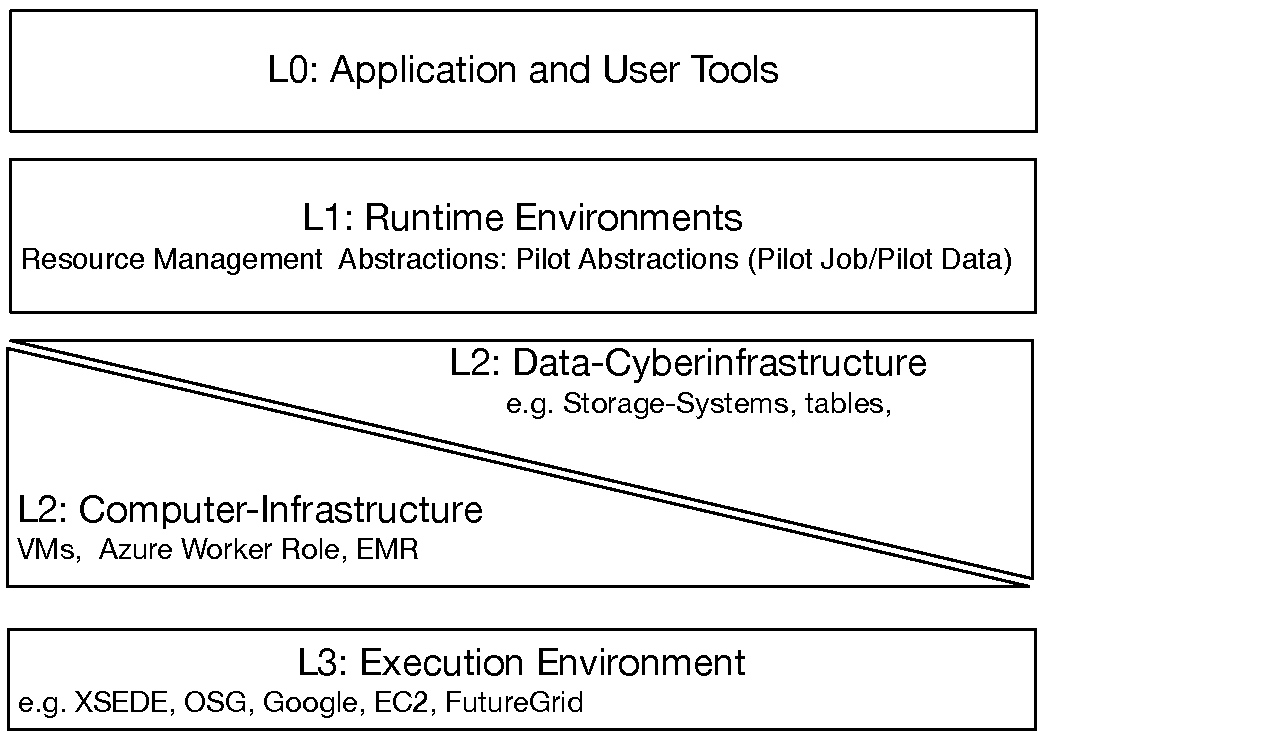
\includegraphics[width=0.6\textwidth]{figures/data-intensive-arch.pdf}
\caption{\jhanote{this figure could even be moved to Section 3. Thoughts?...}}
\label{fig:figures_arch}
\end{figure}



\subsection{Pilot-Abstractions for Clouds: BigJob and BigData}

\alnote{Better P* introduction...}
\alnote{Bring CU, DU, VMs, pilot... How are VMs started through Pilot 
abstractions... - sequence chart?!}
\alnote{Break up 4.3 in compute and data section?}

BigJob and BigData provide a higher-level, unifying interface to heterogeneous
and/or distributed data. The framework is accessed via the
Pilot-API~\cite{pilot_api}, which provides two key abstractions: \pilotjob and
\pilotdata. Applications can specify their resource requirements using a
\pilot description. \pilots are started via the \pilotcomputeservice
respectively the \pilotdataservice.

\pilotjobs eliminate the need to interact with different kinds of compute 
resources, e.\,g.\ batch-style HPC/HTC resources as well as cloud resources, 
and provide a unified abstraction for allocation such resources. Similarly, 
\pilotdata removing the need to interoperate with different data sources and 
stores, e.\,g.\ repositories, databases etc, by providing a virtualized data 
service layer, which can be used to allocated and access a heterogeneous set 
of data sources and stores.

\begin{figure}[t]
	\centering
		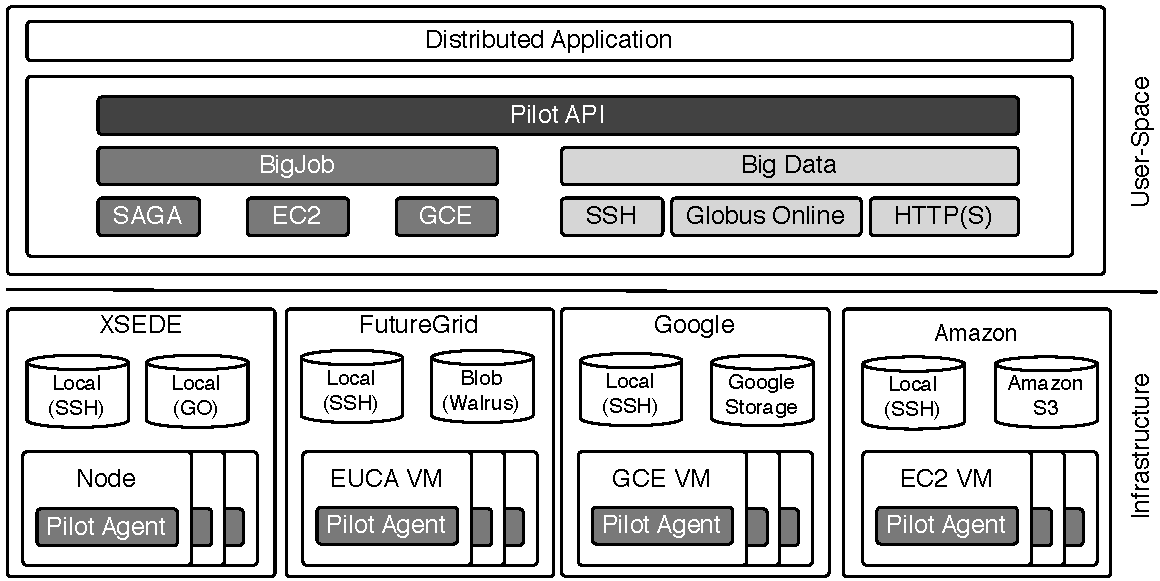
\includegraphics[width=0.7\textwidth]{figures/cloud_pilot_job.pdf}
	\caption{\textbf{Pilot Abstractions and Clouds:} BigJob and BigData 
	provide a unified abstraction to compute and data resources of both grid 
	and cloud environments. Resources are either accessed via 
	SAGA~\cite{ogf-gfd-90,saga-bliss-pd} or via a custom adaptor.}
	\label{fig:figures_cloud_pilot_job}
\end{figure}

Figure~\ref{fig:figures_cloud_pilot_job} shows the different layers of the
architecture. BigJob supports various resource types via a flexible plugin
architecture. In addition to SAGA, BJ can natively utilize both the EC2 and
GCE API to launch BJ agents. The EC2-API~\cite{amazonec2api} is the de facto 
standard for managing VMs in clouds and can also be used for accessing 
different science clouds, e.\,g.\ the Eucalyptus and OpenStack cloud of 
FutureGrid. Google Compute Engine provides modern HTTP/REST/JSON and OAUTH for 
authentication. 

A \pilotdata can be placed on different types of storage, e.\,g.\ a local or
remote filesystem or on object stores as often found in cloud environments. .
Depending on the storage type different access respectively transfer protocols
are supported. For example, local/remote storage both on grid and cloud
resources can be managed via SSH. On production grid infrastructures, such as
XSEDE~\cite{xsede}, this kind of storage can also be accessed via Globus
Online~\cite{10.1109/MIC.2011.64}, which underneath relies on
GridFTP~\cite{ogf-gfd-20} for file movement etc. A particularity of cloud
environments are the described object stores. Object stores are typically
accessed via custom API typically based on HTTP/REST. For example, the Amazon
S3 API~\cite{amazons3api} is based on HTTP and XML and is also supported by
Eucalyptus Walrus and OpenStack Swift.

BigJob and BigData rely on the Boto library~\cite{boto} for accessing storage
and compute resources that provide an Amazon S3 respectively EC2 compliant
interface. The Google cloud adaptors directly access the Google services via
the Google Python API client~\cite{google-api-client}.

 

\jhanote{unclear what HLA here implies} \jhanote{In general I think
  this sub-section can be absorbed. We already have Section 3. Refer
  to parts of it? Move some parts there?}




\subsection{Pilot-API: Managing Data and Compute Dependencies}

Pilot-Abstractions can marshal the difference between the different cloud
storage types and and provide a seamless, unifying environment to the
application simplify the usage of distributed infrastructures. Application can 
acquire resources in form of \pilots. A central \computedataservice is used to 
submit \computeunits (\cus) and \dataunits (\dus) to these pilots. Application 
can declaratively specify \cus and \dus and effectively manage the data flow 
in between. 

\begin{figure}[htbp]
	\centering
		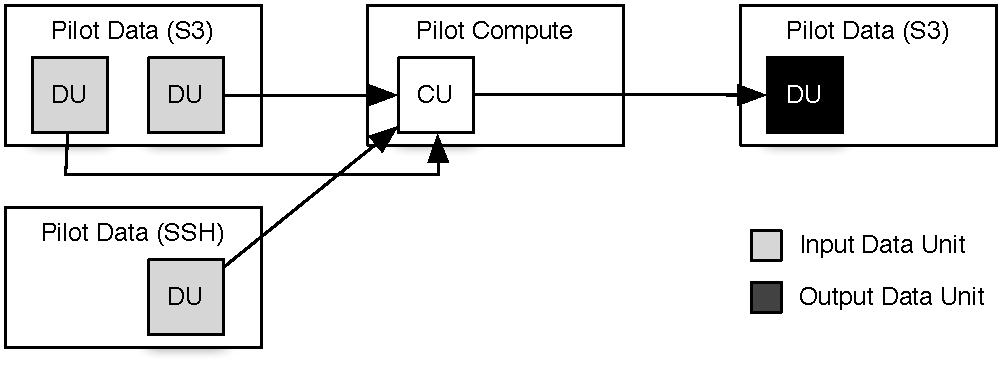
\includegraphics[width=0.7\textwidth]{figures/data-flow.pdf}
	\caption{DU and CU Interactions and Data Flow}
	\label{fig:figures_data-flow}
\end{figure}

Figure~\ref{fig:figures_data-flow} shows the interactions and the data flow
between \computeunits and \dataunits. A \cu can have both input and output
dependencies to a set of \dus. BigJob and BigData will ensure that these
dependencies are met when the \cu is executed, i.\,e.\ either the \dus are
move to the \cu or the \cu is executed at (or close to) the location of the
\dus. The output files can be automatically transferred to a set of output
\dus. Listing~\ref{lst:cu_du_dependencies} shows how these dependencies are
specified on API-level.

\begin{lstlisting}[caption={{Managing \dataunit/\computeunit Dependencies}}, style=myPythonListing, label={lst:cu_du_dependencies}, float=t]
compute_unit_description = {
         "executable": "/bin/cat",
         "arguments": ["test.txt"],
         "number_of_processes": 1,
         "output": "stdout.txt",
         "error": "stderr.txt",   
         "input_data": [input_data_unit.get_url()],
         # Put files stdout.txt and stderr.txt into output data unit
         "output_data": [
                         {
                          output_data_unit.get_url(): 
                          ["std*"]
                         }
                        ]    
}
\end{lstlisting}

T

\alnote{
Distinguish data movement into cloud and intra cloud is important
No shared file system, but S3 as object store (cache)
}


\subsection{Affinities and Scheduling}

\pilot abstraction provide the basis for application-level scheduling.
Applications can make placement decisions based on the \pilots it has
acquired. Additionally, applications can rely on an application-level
scheduling service as provided by BigJob and BigData. This service is exposed
via the \computedataservice interface and accepts both \cus and \dus. The
service decides how and when to place data and schedule its movement.

The framework relies on affinity descriptions for resources and \pilots to 
efficiently manage the different kinds of storage as well as distribution of 
data/compute across WAN. As explained before, even within a single cloud, 
managing data locality is a great challenge due the various storage options. 
Figure~\ref{fig:figures_storage-types} summarized the different kinds of 
storage options an application has to manage. 

\begin{figure}[t]
	\centering
		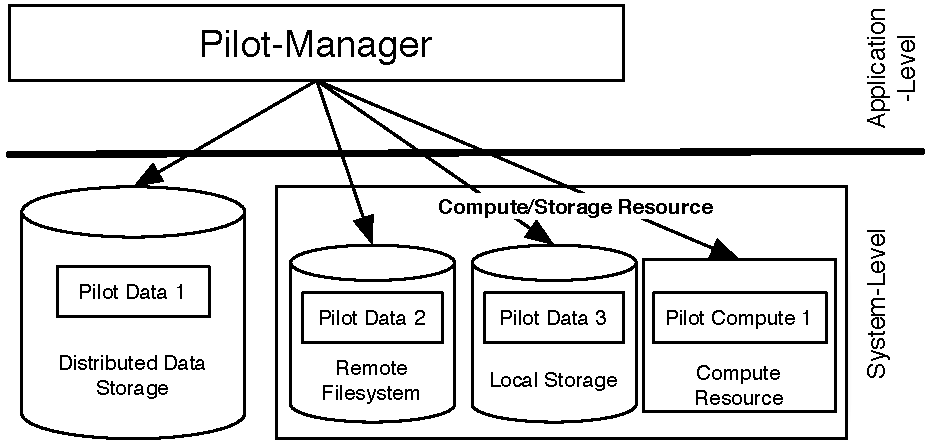
\includegraphics[width=0.6\textwidth]{figures/storage-types.pdf}
                \caption{Pilot-Compute and Pilot-Data on Different
                  Types of Storage Resources}
	\label{fig:figures_storage-types}
\end{figure}



\pilot-abstractions not only provide a uniform interface to these different
kinds of storage, the also support application-level scheduling. The core of
the \pilot-manager is an affinity-aware scheduler. BigJob and BigData support
different forms of data/compute affinities via the \computedataservice. The
internal scheduler of the \computedataservice relies on affinity as first
entity to describe relationships between \dus, \cus and resources. Affinities
are an essential tool for modeling the different storage characteristics and
to allow an effective reasoning about different storage topologies and
data/compute placements.

For this purpose, every resource is assigned an affinity label.
Figure~\ref{fig:figures_affinities} shows how a distributed system consisting
of different types of cloud and grid resources can be modeled. The shorter the 
distance between two nodes, the higher the affinity. Commercial clouds, such 
as Amazon and Google, are typically organized into geographic regions. Within 
each region multiple availability zones exist. Commonly, data movements 
between the lower-level availability zones are cheap and fast, while movements 
between regions costs some significant amount on money and time. Even worse 
are movements between infrastructure, e.\,g.\ between Amazon, Google and 
FutureGrid.


\begin{figure}[t]
	\centering
		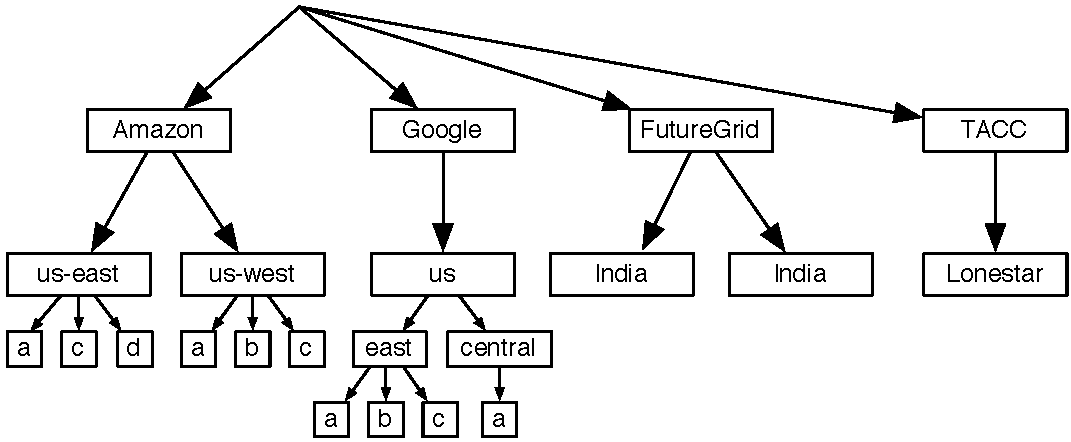
\includegraphics[width=0.6\textwidth]{figures/affinities.pdf}
	\caption{\textbf{Managing Affinities between Cloud and Grid Resources:} \pilotdata assigns each resource an affinity based on a simple hierarchical model.}
	\label{fig:figures_affinities}
\end{figure}

Each of the storage types in figure~\ref{fig:figures_storage-types} can be 
assigned an affinity. The model is able to deal with subtle differences 
between clouds and grids/clouds. For example, at Amazon S3 is service that is 
confined by a single region, while Google Storage spawns multiple regions.

The \computedataservice scheduler matches the affinity requirements of
a \cu/\du with the available set of resources before assigning it to a
\pilot.  \cus are placed closed to a \du. Before a \cu is actually
run, the \du is exported to the working directory of the \cu. In the
cloud cases e.\,g.\ this means that the data is copied from an object
store to the local filesystem where the \cu runs.


\section{Pilot-MapReduce for Clouds}

Pilot-MapReduce (PMR)~\cite{Mantha:2012:PEF:2287016.2287020} is a pilot-based
implementation of the MapReduce programming model, which decouples the
logic/pattern of MapReduce from the actual management of the compute, data and
network resources. By decoupling job scheduling and monitoring from the
resource management, PMR can efficiently reuse the resource management and
late-binding capabilities of BigJob and BigData.

PMR exposes an easy-to-use interface which provides the complete
functionality needed by any MapReduce-based application, while hiding
the more complex functionality, such as chunking of the input, sorting
the intermediate results, managing and coordinating the map and reduce
tasks, etc., these are generically implemented by the
framework.

PMR allocates both storage and compute resources using \pilot abstractions, in
particular the BigJob and BigData implementation. Having spawned a set of
\pilots, PMR can flexibly utilized for them for executing map and reduce tasks
as well as for managing the input, intermediate and output data.


\begin{figure}[t]
	\centering
	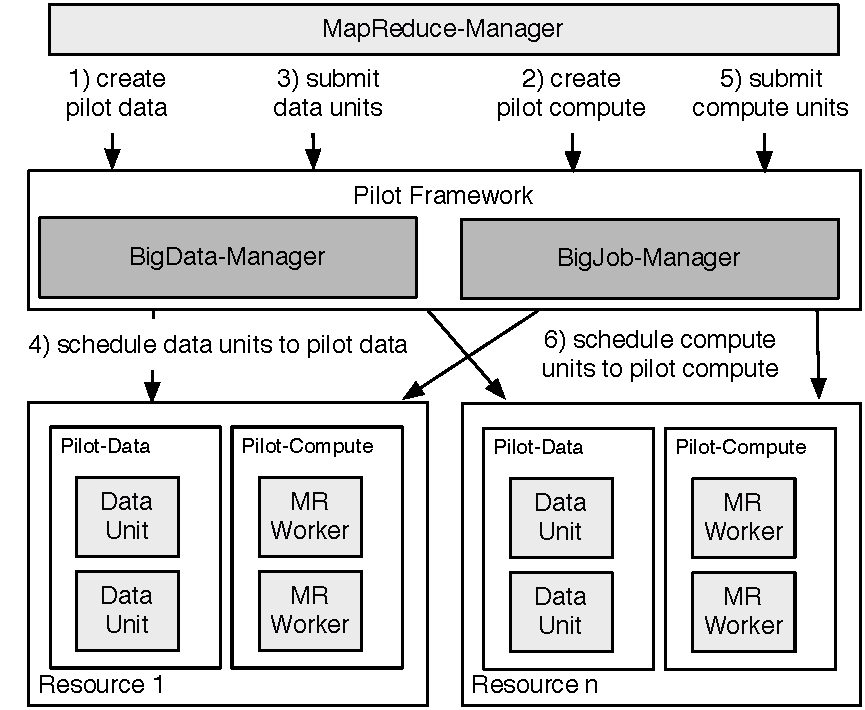
\includegraphics[width=0.5\textwidth]{figures/mr-arch.pdf}
	\caption{\textbf{Pilot-based 
		MapReduce~\cite{Mantha:2012:PEF:2287016.2287020}:} Each pilot (both
          compute and data pilot) can be associated with an affinity
          label. The BigData and BigJob Manager will ensure that CUs
          and DUs are placed with respect to these
          requirements. \jhanote{Figures that have been previously
            used/published need proper citing. I believe this is one of them}}
	\label{fig:figures_mapreduce-pilotdata}
\end{figure}


\alnote{Add layered diagram (incl. PMR) of software stack for different 
infrastructures}
\pmnote{ is it just adding a Pilot-MapReduce layer to Fig:1 ? }

\section{Experiments}

In this section we analyze the performance and scalability of BigJob and 
BigData in different scenarios. For this purpose we run several experiments on 
FutureGrid (FG) and XSEDE. For the purpose of our analysis, we utilize the 
Eucalyptus cloud on India/FutureGrid, Amazon EC2 and Google Compute Engine. 
Each experiment is repeated at least five times.

	
\subsection{Pilot Data on Clouds}

An important challenge when running distributed data-intensive tasks is the 
effective management of data, and its efficient transfer. In the following, we 
investigate the initial phase of staging files to the cloud as well as the 
the cloud-internal overhead of file movements.  In the following, we use the 
FutureGrid hotel as submission machine, i.\,e.\ the machine where the initial 
data resides and the \pilots are submitted from.

In scenario (i) we investigate the execution of 1 \cu, with an input \du of
size 1\,GB. Figure~\ref{fig:performance_pd_google_aws} shows the results.
Typically, data movement into the cloud are more expensive than intra-cloud
data movements. In this particular scenario the data ingest time for clouds
varies between $~$4\,minutes (for Amazon) and $~$18\,minutes. The primary
determinant of this time is the available Internet bandwidth. Once the data is
in the cloud, it can be re-used multiple times. While the ingest performance
is determined by external factors (currently utilization of the Internet
connection), in the investigated scenario the data transfer time is
consistently higher Google Compute Engine than for Amazon. The external
dependency on Internet bandwidth is the high standard deviation (that is
mainly caused by the data ingest phase). Also, it must be noted that Amazon
gives you more option to select a location for your data -- in this scenario
the region us-east, which is close to the hotel resource, was used. For Google 
Storage it is only possible to select between the US and Europe.

With respect to the \pilot startup time (which includes the VM startup time), 
GCE is clearly faster than Amazon EC2. Also, the available intra-cloud 
bandwidths are much better for GCE: The data download time for GS/GCE is about 
40\,\% faster than for S3/EC2. Also, the \cu execution time are significantly 
lower on GCE. In both cases the smallest possible VM was used; however, it 
must be noted that Amazon's t1.micro instance type doesn't provide any 
guaranteed CPU time. Also the memory is with 613\,MB considerable smaller than 
for Google's smallest VM n1-standard-1, which has 3.75\,GB memory.

\jhanote{I know you'll do it but just as a
  note: Don't forget to mention the number of times the experiment is
  repeated, else difficult to get a sense/infer what error bars 
imply}\alnote{added above. maybe we have to give different numbers for PMR and 
initial measurements}
\begin{figure}[htbp]
	\centering
		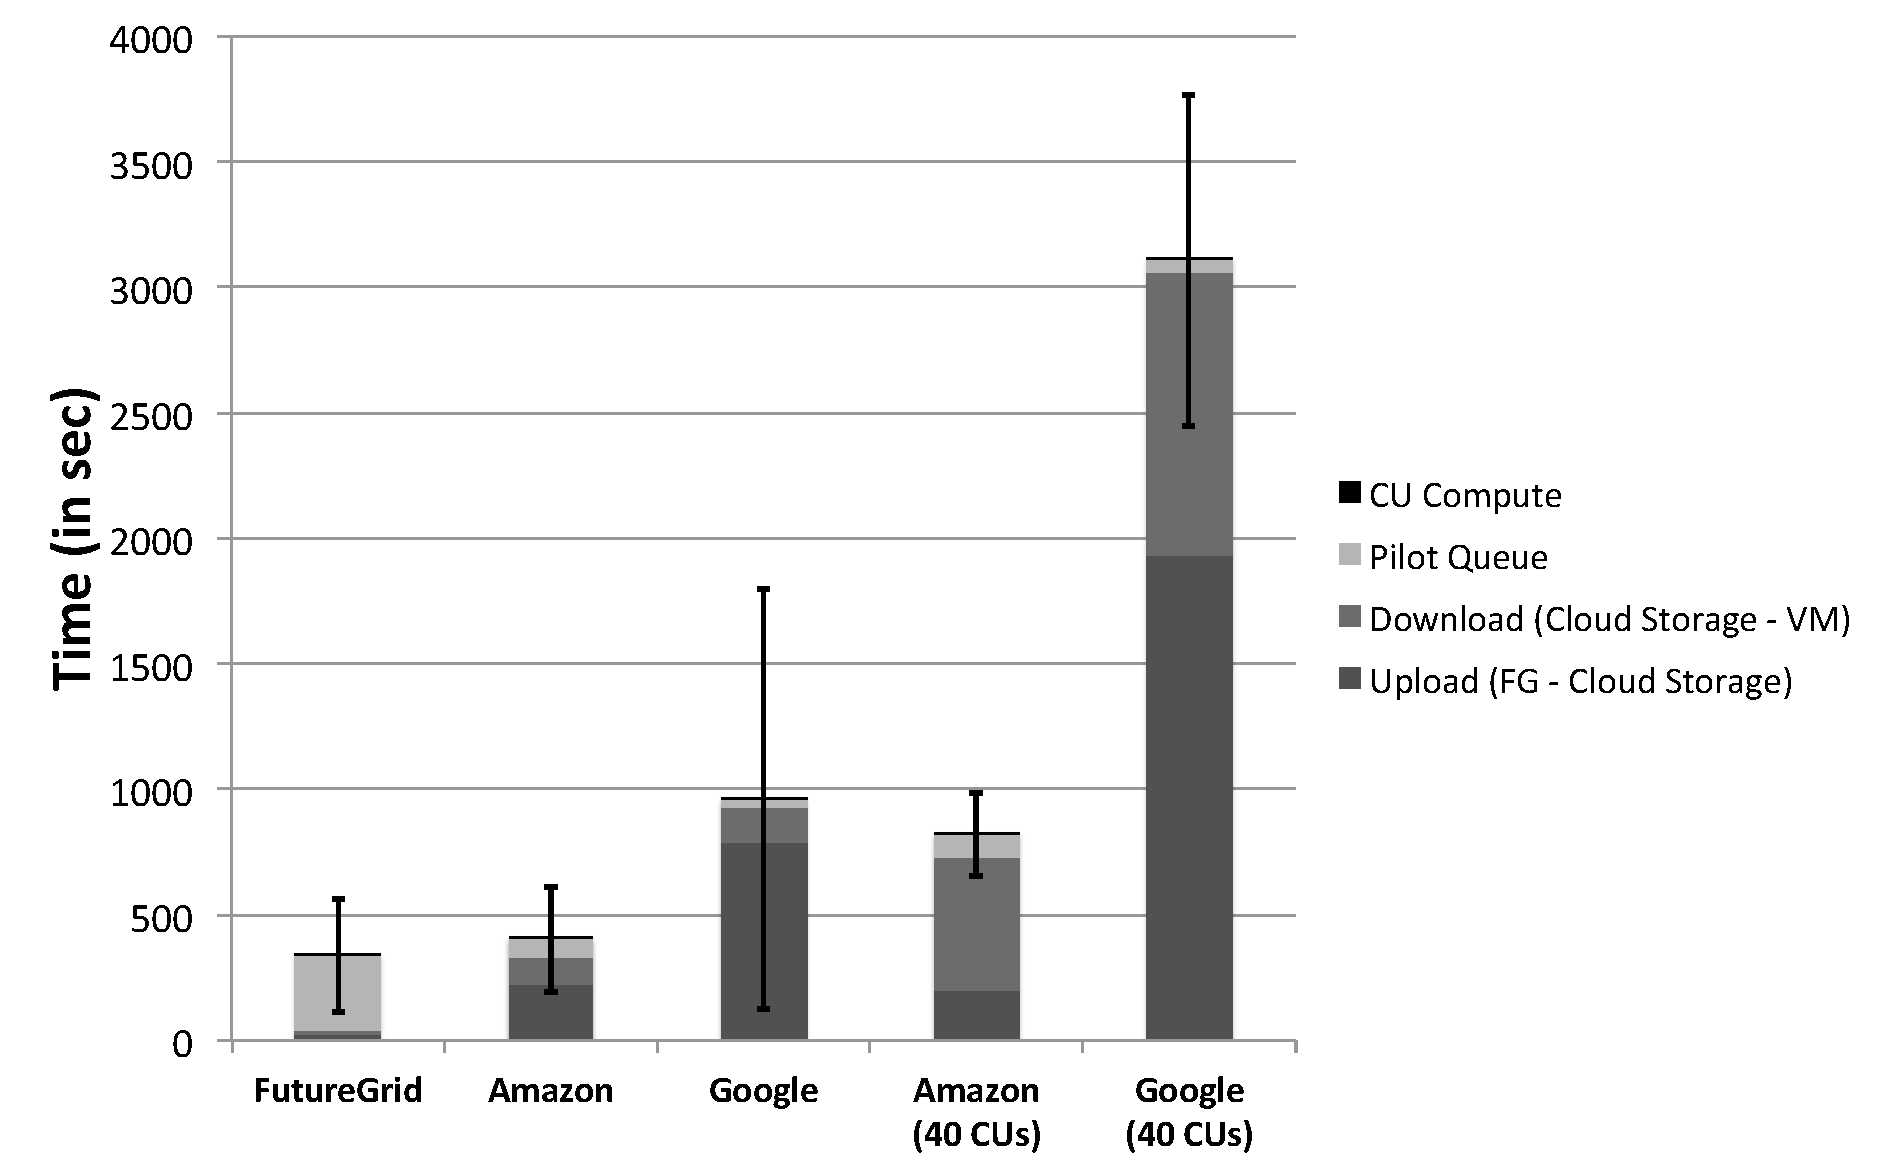
\includegraphics[width=0.75\textwidth]{performance/pd_google_aws.pdf}
	\caption{\textbf{Performance of BigJob and BigData on Different Resource Types}}
	\label{fig:performance_pd_google_aws}
\end{figure}



Experiments:
\begin{itemize}
	\item Scale input data: 1\,GB, 10GB, 100GB, 1000 GB
	\item Number of Resources: 1, 2, 4, 8, 16, 32 VMs
	\item Number of CUs
	\item Size of VMs vs. startup time...
\end{itemize}



\subsection{Pilot-MapReduce}
\begin{itemize}
	\item grid only
	\item cloud only
	\item grid / cloud concurrently
	\item  Different amounts of intermediate data: 1GB, 10GB, 100GB, 1000 GB	
\end{itemize}

\section{Conclusion and Future Work}

Extend to other data-intensive abstractions

\bibliographystyle{wileyj}
\bibliography{literatur,saga,saga-related,local}

\end{document}
